\documentclass{standalone}
\usepackage[utf8]{inputenc}
\usepackage{pgfplots}
\DeclareUnicodeCharacter{2212}{−}
\usepgfplotslibrary{groupplots,dateplot}
\usetikzlibrary{patterns,shapes.arrows}
\pgfplotsset{compat=newest}
\begin{document}
% This file was created with tikzplotlib v0.10.1.
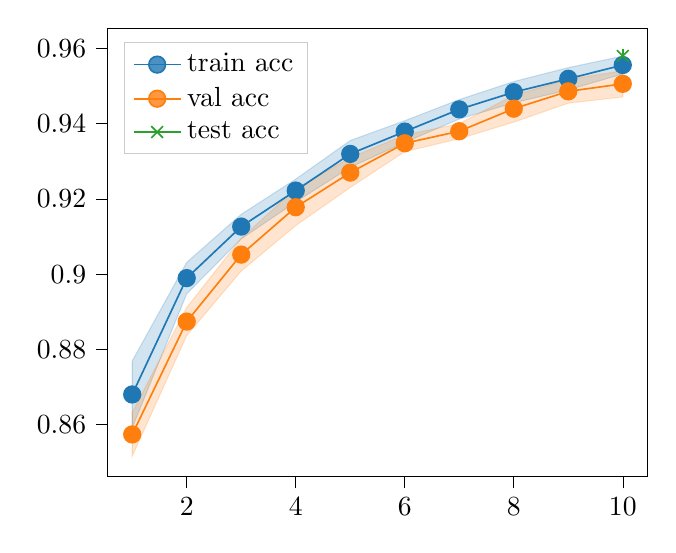
\begin{tikzpicture}

\definecolor{darkgray176}{RGB}{176,176,176}
\definecolor{darkorange25512714}{RGB}{255,127,14}
\definecolor{forestgreen4416044}{RGB}{44,160,44}
\definecolor{lightgray204}{RGB}{204,204,204}
\definecolor{steelblue31119180}{RGB}{31,119,180}

\begin{axis}[
legend cell align={left},
legend style={
  fill opacity=0.8,
  draw opacity=1,
  text opacity=1,
  at={(0.03,0.97)},
  anchor=north west,
  draw=lightgray204
},
tick align=outside,
tick pos=left,
x grid style={darkgray176},
xmin=0.55, xmax=10.45,
xtick style={color=black},
y grid style={darkgray176},
ymin=0.846199867094401, ymax=0.965384189027827,
ytick style={color=black}
]
\path [draw=steelblue31119180, fill=steelblue31119180, opacity=0.2]
(axis cs:1,0.876899302005768)
--(axis cs:1,0.85914808511734)
--(axis cs:2,0.894768118858337)
--(axis cs:3,0.909394383430481)
--(axis cs:4,0.919185876846313)
--(axis cs:5,0.928398966789246)
--(axis cs:6,0.935037016868591)
--(axis cs:7,0.941233575344086)
--(axis cs:8,0.945551753044128)
--(axis cs:9,0.948976218700409)
--(axis cs:10,0.953238904476166)
--(axis cs:10,0.957967936992645)
--(axis cs:10,0.957967936992645)
--(axis cs:9,0.954908549785614)
--(axis cs:8,0.951207518577576)
--(axis cs:7,0.946400344371796)
--(axis cs:6,0.940793514251709)
--(axis cs:5,0.935526371002197)
--(axis cs:4,0.925261497497559)
--(axis cs:3,0.915907382965088)
--(axis cs:2,0.903136849403381)
--(axis cs:1,0.876899302005768)
--cycle;

\path [draw=darkorange25512714, fill=darkorange25512714, opacity=0.2]
(axis cs:1,0.863182783126831)
--(axis cs:1,0.851617336273193)
--(axis cs:2,0.883679866790771)
--(axis cs:3,0.90084570646286)
--(axis cs:4,0.912925660610199)
--(axis cs:5,0.923050403594971)
--(axis cs:6,0.932572841644287)
--(axis cs:7,0.936000049114227)
--(axis cs:8,0.940422356128693)
--(axis cs:9,0.945463120937347)
--(axis cs:10,0.947101533412933)
--(axis cs:10,0.954098641872406)
--(axis cs:10,0.954098641872406)
--(axis cs:9,0.951736867427826)
--(axis cs:8,0.947577774524689)
--(axis cs:7,0.939999997615814)
--(axis cs:6,0.937027096748352)
--(axis cs:5,0.930949687957764)
--(axis cs:4,0.922674477100372)
--(axis cs:3,0.909554302692413)
--(axis cs:2,0.891120314598083)
--(axis cs:1,0.863182783126831)
--cycle;

\addplot [semithick, steelblue31119180, mark=*, mark size=3, mark options={solid}]
table {%
1 0.868023693561554
2 0.898952484130859
3 0.912650883197784
4 0.922223687171936
5 0.931962668895721
6 0.93791526556015
7 0.943816959857941
8 0.948379635810852
9 0.951942384243011
10 0.955603420734406
};
\addlegendentry{train acc}
\addplot [semithick, darkorange25512714, mark=*, mark size=3, mark options={solid}]
table {%
1 0.857400059700012
2 0.887400090694427
3 0.905200004577637
4 0.917800068855286
5 0.927000045776367
6 0.93479996919632
7 0.938000023365021
8 0.944000065326691
9 0.948599994182587
10 0.95060008764267
};
\addlegendentry{val acc}
\path [draw=forestgreen4416044, semithick]
(axis cs:10,0.956033288734034)
--(axis cs:10,0.959966719849035);

\addplot [semithick, forestgreen4416044, mark=x, mark size=3, mark options={solid}]
table {%
10 0.958000004291534
};
\addlegendentry{test acc}
\end{axis}

\end{tikzpicture}

\end{document}